% Set the document's formatting to "report"
\documentclass[openright]{report}

% Include titlesec[personalized chapters], graphicx[images], tocbibind[bibliography in toc], comment[comment paragraphs], lmodern/fontend[fix tilde typesetting], afterpage[insert blankpages], etoolbox[flawless page numbering], blindtext[lorem ipsum], mathtools[math symbols], listings/alloy/color[alloy syntax], fp[variables evaluation] and glossaries/imakeidx[glossary] packages
\usepackage[utf8]{inputenc}
\usepackage{titlesec}
\usepackage{graphicx}
\usepackage{tocbibind}
\usepackage{comment}
\usepackage{lmodern}
\usepackage[T1]{fontenc}
\usepackage{afterpage}
\usepackage{etoolbox}
\usepackage{blindtext}
\usepackage{mathtools}
\usepackage{listings}
\usepackage[nomessages]{fp}
\usepackage[nonumberlist,acronym,toc,xindy]{glossaries}
\makeglossaries
\usepackage[xindy]{imakeidx}
\makeindex


% Patch page numbering
\patchcmd{\abstract}{\titlepage}{\thispagestyle{empty}}{}{}
\patchcmd{\endabstract}{\endtitlepage}{\clearpage}{}{}

% Create new \blankpage command
\newcommand\blankpage{%
    \null
    \thispagestyle{empty}%
    \addtocounter{page}{-1}%
    \newpage}

% Edit title styling
\titleformat{\chapter}{\Huge\bfseries}{}{0pt}{\Huge}

% Set images path
\graphicspath{{../resources/images/}}

% Create auxiliary variables for worktime and version tracking 
\def \worktimeNicola {0}
\def \worktimeGiacomo {0}
\FPupn{worktimeTotal}{worktimeNicola worktimeGiacomo + 0 round}
\FPupn{version}{0.1}


\begin{document}

	\begin{titlepage}
		\centering

\includegraphics[width=0.50\textwidth]{polimi}\\\vspace{0.25cm}
{\scshape\LARGE Politecnico di Milano\par}\vspace{0.25cm}
{\scshape\Large Software Engineering II project: PowerEnjoy\par}\vspace{1.5cm}
{\huge\bfseries Code Inspection \par}\vspace{1cm}
{\large Gregori Giacomo and Ruaro Nicola\par}\vfill

% Bottom of the page
{\large \today \\Version \version}

	\end{titlepage}

	% Change page numbering to uppercase roman for introductory pages
    \pagenumbering{Roman}

    \tableofcontents

    \newpage
    \blankpage
    \begin{abstract}
		This document provides a detailed description of the Integration Test's planning for the PowerEnJoy system. It is based on the RASD and DD documents presented in the previous deliveries and must explain to the developement team how to test the system.

	\end{abstract}

	% Change page numbering to arabic for the rest of the document
	\pagenumbering{arabic}

    \chapter{Introduction}
    	\section{Scope of the System}
PowerEnJoy is a car-sharing service based on mobile and web applications which should allow users to reserve vehicles and use them.
\\TODO: brief architecture/algorithms/UI description
\section{Document Structure}
\begin{description} 
	\item[Introduction: ] In this chapter an introduction to the system and the Design Document is given.
	\item[Architectural Design: ] In this section an overall description of the architecture is given, it is structured into N different parts: 
		\begin{itemize}
			\item Overview: High-level components and their interaction
			\item Component view
			\item Deployment view
			\item Runtime view
			\item Component Interfaces
			\item Selected architectural styles and patterns
			\item Other design decisions
		\end{itemize}
	\item[Algorithm Design: ] In this chapter the implemented algorithms are discussed and presented using flow-charts and pseudo-code in order to ease the comprehension and focus on the functionality.
	\item[User Interface Design: ] In this section the main choices in User Interface and User Experience design are discussed.
	\item[Requirements Traceability: ] In this section a clear link between requirements specification (RASD) and design decisions (DD) is created.
\end{description}

	\chapter{Integration strategy}
		\section{Entry criteria}
Before proceeding with the integration test in this section we analysed the prerequisites that the software must satisfy.
\\First of all we must have a code-complete project, all modules must be available and their performances and memory requirements have to fit the specifications.
\\Secondly all the modules must be unit tested. 
\\Finally the RASD and DD must be completed, they provide all the documentation that we need for proceeding in the succeeding steps.

\section{Elements to be integrated}
In the Design Document, we identified four main Tiers: the EIS Tier, the Business Tier, the Web Tier and the Client Tier. These are the subsystems that we must integrate in this section.
\\The Enterprise Information System Tier is composed principally by a DBMS that has to be integrated while in the Business Tier all the system components have to be tested individually before to be integrated. The Web Tier relates to the Client Tier and the Business Tier and both the interfaces have to be integrated. Finally, the Client Tier is composed by the On-Board computer, the Mobile application and Web application; they have to be tested individually and then they have to be integrated with their respective Tier. 

\section{Integration testing strategy}
We choose for our integration testing strategy to adopt a bottom-up approach. In this way, we test the subsystems from the lower level to the top level, where all the modules are integrated. 
\\There are different advantages following this strategy. The test conditions for each module are easier to create and the test results can be analysed in a simpler way. Then it's easier to localize problems and faults. In the end we can proceed with the test phase of our subsystems alongside their implementation.
\\On the other side the bottom-up approach brings some disadvantages. The main one is the need of driver programs in order to simulate the missing modules while they aren't already deployed. Another point is the fact that we can't test the whole program until the last module has been developed. Anyway, we think that these disadvantages are bearable comparing the advantages that this approach provides, a last evidence is the fact that probably almost all the faults occurs toward the bottom of the system.
\\In the testing phase we also selected the order of the subsystems to analyse, not randomly but privileging the critical ones.
\\ We also follow a specific path before performing the integration test. First of all, we design the integration test and the specific drivers if they aren't already done. If it was not made at the unit test we design the input test data, thirdly we set the modules involved, the drivers and the input test data. Finally, we proceed performing the integration test.

\section{Sequence of Component/Function Integration}
NOTE: The structure of this section may vary depending on the integration strategy you select in Section 2.3. Use the structure proposed below as a non mandatory guide.

	\newpage
	\subsection{Software Integration Sequence}
	The following figures (fig.\ref{fig:database_integration}, fig.\ref{fig:application_logic_subsystem}) show the components of the PowerEnJoy system integrated into subsystems, the arrows indicate the order of integration.

	\begin{figure}[!ht]
	  \centering
	  \vspace{0.2cm}
	  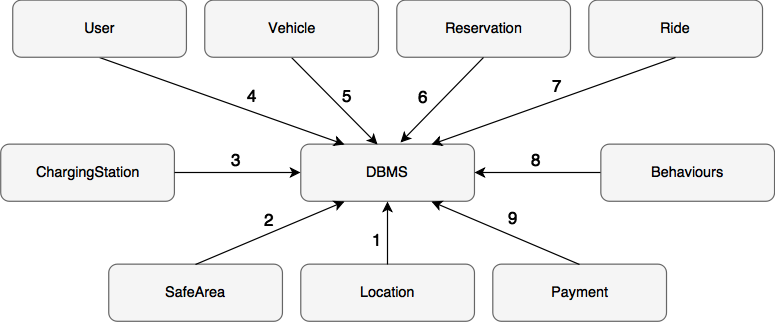
\includegraphics[width=1.0\textwidth]{/ITPD/database_subsystem}\\
	  \vspace{0.2cm}
	  \caption{Integration sequence for the Enterprise-Information-System subsystem} 
	  \label{fig:database_integration} 
	\end{figure}

	\begin{center}
		\vspace{0.6cm}
		\begin{tabular}{|l|l|l|}
			\hline
			\textbf{ID} & \textbf{Integration Test} & \textbf{Paragraphs} \bigstrut \\\hline
			\hline
			I01 & Location \ensuremath{\rightarrow} DB & \ref{I01}  \ref{TP1} \bigstrut \\\hline
			I02 & SafeArea \ensuremath{\rightarrow} DB & \ref{I02}  \ref{TP1} \bigstrut \\\hline
			I03 & ChargingStation \ensuremath{\rightarrow} DB & \ref{I03}  \ref{TP1} \bigstrut \\\hline
			I04 & User \ensuremath{\rightarrow} DB & \ref{I04}  \ref{TP1} \bigstrut \\\hline
			I05 & Vehicle \ensuremath{\rightarrow} DB & \ref{I05}  \ref{TP1} \bigstrut \\\hline
			I06 & Reservation \ensuremath{\rightarrow} DB & \ref{I06}  \ref{TP1} \bigstrut \\\hline
			I07 & Ride \ensuremath{\rightarrow} DB & \ref{I07}  \ref{TP1} \bigstrut \\\hline
			I08 & Behaviours \ensuremath{\rightarrow} DB & \ref{I08}  \ref{TP1} \bigstrut \\\hline
			I09 & Payment \ensuremath{\rightarrow} DB & \ref{I09}  \ref{TP1} \bigstrut \\\hline
		\end{tabular}
	\end{center}

	\newpage
	\begin{figure}[!ht]
	  \centering
	  \vspace{0.2cm}
	  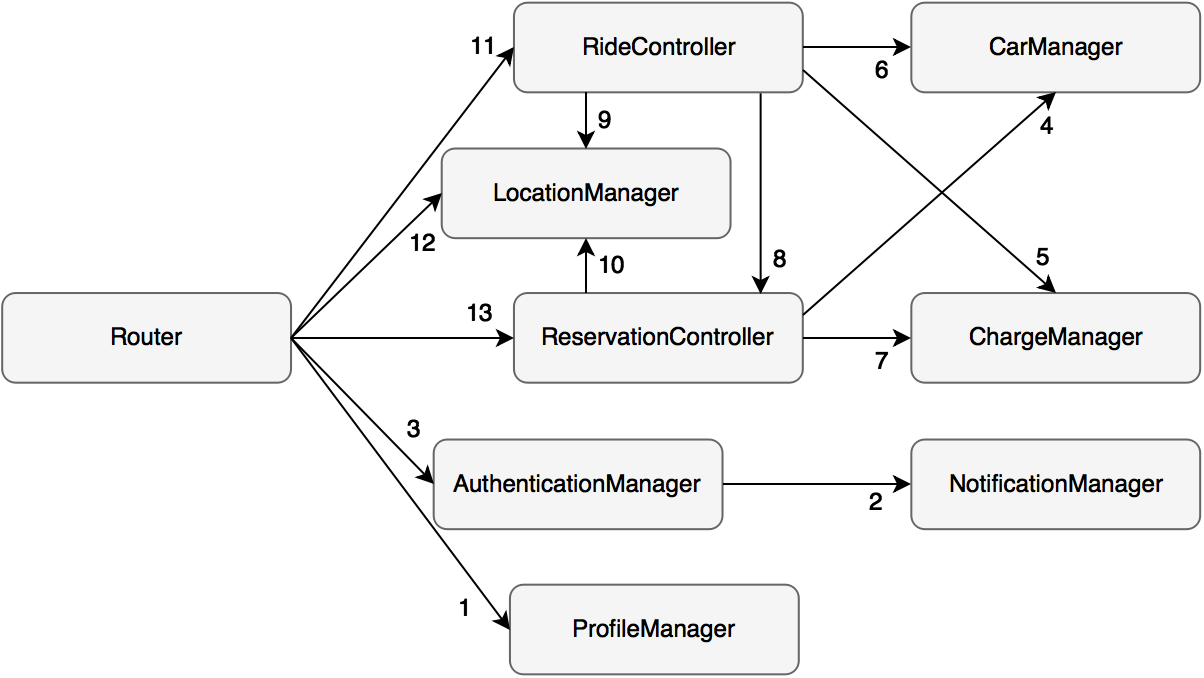
\includegraphics[width=1.0\textwidth]{/ITPD/application_logic_subsystem}\\
	  \vspace{0.2cm}
	  \caption{Integration sequence for the Business subsystem} 
	  \label{fig:application_logic_subsystem} 
	\end{figure}

	\begin{center}
		\vspace{0.6cm}
		\begin{tabular}{|l|l|l|}
			\hline
			\textbf{ID} & \textbf{Integration Test} & \textbf{Paragraphs} \bigstrut \\\hline
			\hline
			I10 & Router \ensuremath{\rightarrow} ProfileManager & \ref{I10}  \ref{TP2} \bigstrut \\\hline
			I11 & AuthenticationManager \ensuremath{\rightarrow} NotificationManager & \ref{I11}  \ref{TP2} \bigstrut \\\hline
			I12 & Router \ensuremath{\rightarrow} AuthenticationManager & \ref{I12}  \ref{TP2} \bigstrut \\\hline
			I13 & ReservationController \ensuremath{\rightarrow} CarManager & \ref{I13}  \ref{TP2} \bigstrut \\\hline
			I14 & RideController \ensuremath{\rightarrow} ChargeManager & \ref{I14}  \ref{TP2} \bigstrut \\\hline
			I15 & RideController \ensuremath{\rightarrow} CarManager & \ref{I15}  \ref{TP2} \bigstrut \\\hline
			I16 & ReservationController \ensuremath{\rightarrow} ChargeManager & \ref{I16}  \ref{TP2} \bigstrut \\\hline
			I17 & RideController \ensuremath{\rightarrow} ReservationController & \ref{I17}  \ref{TP2} \bigstrut \\\hline
			I18 & RideController \ensuremath{\rightarrow} LocationManager & \ref{I18}  \ref{TP2} \bigstrut \\\hline
			I19 & ReservationController \ensuremath{\rightarrow} LocationManager & \ref{I19}  \ref{TP2} \bigstrut \\\hline
			I20 & Router \ensuremath{\rightarrow} RideController & \ref{I20}  \ref{TP2} \bigstrut \\\hline
			I21 & Router \ensuremath{\rightarrow} LocationManager & \ref{I21}  \ref{TP2} \bigstrut \\\hline
			I22 & Router \ensuremath{\rightarrow} ReservationController & \ref{I22}  \ref{TP2} \bigstrut \\\hline
		\end{tabular}
	\end{center}

	\newpage
	\subsection{Subsystem Integration Sequence}
	Figure \ref{fig:subsystem_integration_sequence} the order in which the subsystems will be integrated.

	\begin{figure}[!ht]
	  \centering
	  \vspace{0.2cm}
	  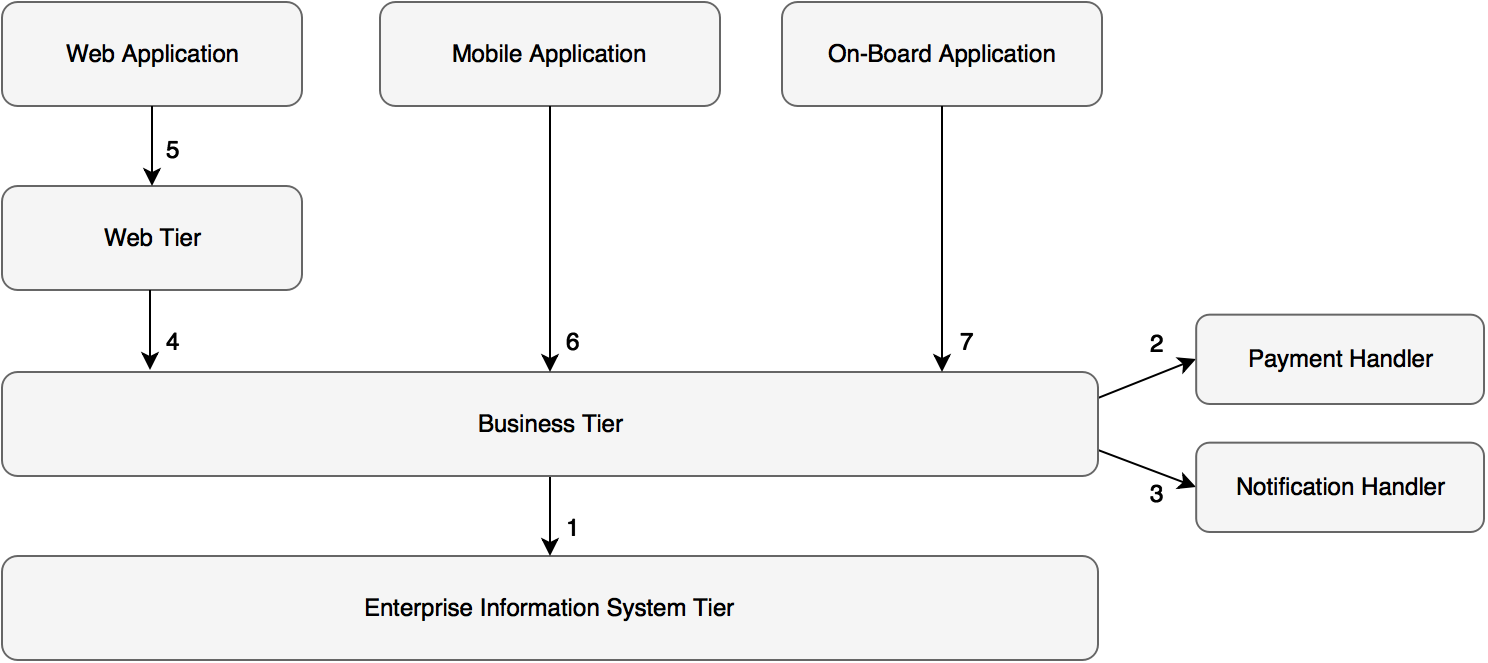
\includegraphics[width=1.0\textwidth]{/ITPD/subsystem_integration_sequence}\\
	  \vspace{0.2cm}
	  \caption{Integration sequence for the subsystems} 
	  \label{fig:subsystem_integration_sequence} 
	\end{figure}


    \chapter{Individual steps and test description}
    	For each step of the integration process identified above, describe the type of tests that will be used to verify that the elements integrated in this step perform as expected. Describe in general the expected results of the test set. You may refer to Chapter 3 and Chapter 4 of the test plan example [1] as an example of what we expect.
(NOTE: This is not a detailed description of test protocols. Think of this as the test design phase. Specific protocols will be written to fulfill the goals of the tests identified in this section.)

\section{Sample Integration test case I01}\label{I01}
\begin{center}
	\vspace{0.6cm}
	\begin{tabular}{|l|l|}
		\hline
		\textbf{Test Case Identifier} & I01T1 \bigstrut \\\hline
		\textbf{Test Item(s)} & Location \ensuremath{\rightarrow} DB \bigstrut \\\hline
		\textbf{Input Specification} & Create typical Location input \bigstrut \\\hline
		\textbf{Output Specification} & Check if the correct functions are called in the DB \bigstrut \\\hline
		\textbf{Environmental Needs} & N/A \bigstrut \\\hline
	\end{tabular}
\end{center}

\section{Sample Integration test case I02}\label{I02}
\begin{center}
	\vspace{0.6cm}
	\begin{tabular}{|l|l|}
		\hline
		\textbf{Test Case Identifier} & I02T1 \bigstrut \\\hline
		\textbf{Test Item(s)} & SafeArea \ensuremath{\rightarrow} DB \bigstrut \\\hline
		\textbf{Input Specification} & Create typical SafeArea input \bigstrut \\\hline
		\textbf{Output Specification} & Check if the correct functions are called in the DB \bigstrut \\\hline
		\textbf{Environmental Needs} & I1 succeeded\bigstrut \\\hline
	\end{tabular}
\end{center}

\section{Sample Integration test case I03}\label{I03}
\begin{center}
	\vspace{0.6cm}
	\begin{tabular}{|l|l|}
		\hline
		\textbf{Test Case Identifier} & I03T1 \bigstrut \\\hline
		\textbf{Test Item(s)} & ChargingStation \ensuremath{\rightarrow} DB \bigstrut \\\hline
		\textbf{Input Specification} & Create typical ChargingStation input \bigstrut \\\hline
		\textbf{Output Specification} & Check if the correct functions are called in the DB \bigstrut \\\hline
		\textbf{Environmental Needs} & I1 succeeded\bigstrut \\\hline
	\end{tabular}
\end{center}

\section{Sample Integration test case I04}\label{I04}
\begin{center}
	\vspace{0.6cm}
	\begin{tabular}{|l|l|}
		\hline
		\textbf{Test Case Identifier} & I04T1 \bigstrut \\\hline
		\textbf{Test Item(s)} & User \ensuremath{\rightarrow} DB \bigstrut \\\hline
		\textbf{Input Specification} & Create typical User input \bigstrut \\\hline
		\textbf{Output Specification} & Check if the correct functions are called in the DB \bigstrut \\\hline
		\textbf{Environmental Needs} & I1 succeeded\bigstrut \\\hline
	\end{tabular}
\end{center}

\section{Sample Integration test case I05}\label{I05}
\begin{center}
	\vspace{0.6cm}
	\begin{tabular}{|l|l|}
		\hline
		\textbf{Test Case Identifier} & I05T1 \bigstrut \\\hline
		\textbf{Test Item(s)} & Vehicle \ensuremath{\rightarrow} DB \bigstrut \\\hline
		\textbf{Input Specification} & Create typical Vehicle input \bigstrut \\\hline
		\textbf{Output Specification} & Check if the correct functions are called in the DB \bigstrut \\\hline
		\textbf{Environmental Needs} & I1 succeeded\bigstrut \\\hline
	\end{tabular}
\end{center}

\section{Sample Integration test case I06}\label{I06}
\begin{center}
	\vspace{0.6cm}
	\begin{tabular}{|l|l|}
		\hline
		\textbf{Test Case Identifier} & I06T1 \bigstrut \\\hline
		\textbf{Test Item(s)} & Reservation \ensuremath{\rightarrow} DB \bigstrut \\\hline
		\textbf{Input Specification} & Create typical Reservation input \bigstrut \\\hline
		\textbf{Output Specification} & Check if the correct functions are called in the DB \bigstrut \\\hline
		\textbf{Environmental Needs} & I4 and I5 succeeded\bigstrut \\\hline
	\end{tabular}
\end{center}

\section{Sample Integration test case I07}\label{I07}
\begin{center}
	\vspace{0.6cm}
	\begin{tabular}{|l|l|}
		\hline
		\textbf{Test Case Identifier} & I07T1 \bigstrut \\\hline
		\textbf{Test Item(s)} & Ride \ensuremath{\rightarrow} DB \bigstrut \\\hline
		\textbf{Input Specification} & Create typical Ride input \bigstrut \\\hline
		\textbf{Output Specification} & Check if the correct functions are called in the DB \bigstrut \\\hline
		\textbf{Environmental Needs} & I1, I4, I5 and I6 succeeded. Payment Driver\bigstrut \\\hline
	\end{tabular}
\end{center}

\section{Sample Integration test case I08}\label{I08}
\begin{center}
	\vspace{0.6cm}
	\begin{tabular}{|l|l|}
		\hline
		\textbf{Test Case Identifier} & I08T1 \bigstrut \\\hline
		\textbf{Test Item(s)} & Behaviour \ensuremath{\rightarrow} DB \bigstrut \\\hline
		\textbf{Input Specification} & Create typical Behaviour input \bigstrut \\\hline
		\textbf{Output Specification} & Check if the correct functions are called in the DB \bigstrut \\\hline
		\textbf{Environmental Needs} & I7 succeeded \bigstrut \\\hline
	\end{tabular}
\end{center}

\section{Sample Integration test case I09}\label{I09}
\begin{center}
	\vspace{0.6cm}
	\begin{tabular}{|l|l|}
		\hline
		\textbf{Test Case Identifier} & I09T1 \bigstrut \\\hline
		\textbf{Test Item(s)} & Payment \ensuremath{\rightarrow} DB \bigstrut \\\hline
		\textbf{Input Specification} & Create typical Payment input \bigstrut \\\hline
		\textbf{Output Specification} & Check if the correct functions are called in the DB \bigstrut \\\hline
		\textbf{Environmental Needs} & I4, I6 and I7 succeeded \bigstrut \\\hline
	\end{tabular}
\end{center}

\section{Sample Integration test case I10}\label{I10}
\begin{center}
	\vspace{0.6cm}
	\begin{tabular}{|l|l|}
		\hline
		\textbf{Test Case Identifier} & I10T1 \bigstrut \\\hline
		\textbf{Test Item(s)} & Router \ensuremath{\rightarrow} ProfileManager \bigstrut \\\hline
		\textbf{Input Specification} & Create typical Router input \bigstrut \\\hline
		\textbf{Output Specification} & Check if the correct functions are called in the ProfileManager \bigstrut \\\hline
		\textbf{Environmental Needs} & N/A \bigstrut \\\hline
	\end{tabular}
\end{center}

\section{Sample Integration test case I11}\label{I11}
\begin{center}
	\vspace{0.6cm}
	\begin{tabular}{|l|l|}
		\hline
		\textbf{Test Case Identifier} & I11T1 \bigstrut \\\hline
		\textbf{Test Item(s)} & AuthenticationManager \ensuremath{\rightarrow} NotificationManager \bigstrut \\\hline
		\textbf{Input Specification} & Create typical AuthenticationManager input \bigstrut \\\hline
		\textbf{Output Specification} & Check if the correct functions are called in the NotificationManager \bigstrut \\\hline
		\textbf{Environmental Needs} & N/A \bigstrut \\\hline
	\end{tabular}
\end{center}

\section{Sample Integration test case I12}\label{I12}
\begin{center}
	\vspace{0.6cm}
	\begin{tabular}{|l|l|}
		\hline
		\textbf{Test Case Identifier} & I12T1 \bigstrut \\\hline
		\textbf{Test Item(s)} & Router \ensuremath{\rightarrow} AuthenticationManager \bigstrut \\\hline
		\textbf{Input Specification} & Create typical Router input \bigstrut \\\hline
		\textbf{Output Specification} & Check if the correct functions are called in the AuthenticationManager \bigstrut \\\hline
		\textbf{Environmental Needs} & I11 succeeded \bigstrut \\\hline
	\end{tabular}
\end{center}

\section{Sample Integration test case I13}\label{I13}
\begin{center}
	\vspace{0.6cm}
	\begin{tabular}{|l|l|}
		\hline
		\textbf{Test Case Identifier} & I13T1 \bigstrut \\\hline
		\textbf{Test Item(s)} & ReservationController \ensuremath{\rightarrow} CarManager \bigstrut \\\hline
		\textbf{Input Specification} & Create typical ReservationController input \bigstrut \\\hline
		\textbf{Output Specification} & Check if the correct functions are called in the CarManager \bigstrut \\\hline
		\textbf{Environmental Needs} & N/A \bigstrut \\\hline
	\end{tabular}
\end{center}

\section{Sample Integration test case I14}\label{I14}
\begin{center}
	\vspace{0.6cm}
	\begin{tabular}{|l|l|}
		\hline
		\textbf{Test Case Identifier} & I14T1 \bigstrut \\\hline
		\textbf{Test Item(s)} & RideController \ensuremath{\rightarrow} ChargeManager \bigstrut \\\hline
		\textbf{Input Specification} & Create typical RideController input \bigstrut \\\hline
		\textbf{Output Specification} & Check if the correct functions are called in the ChargeManager \bigstrut \\\hline
		\textbf{Environmental Needs} & N/A \bigstrut \\\hline
	\end{tabular}
\end{center}

\section{Sample Integration test case I15}\label{I15}
\begin{center}
	\vspace{0.6cm}
	\begin{tabular}{|l|l|}
		\hline
		\textbf{Test Case Identifier} & I15T1 \bigstrut \\\hline
		\textbf{Test Item(s)} & RideController \ensuremath{\rightarrow} CarManager \bigstrut \\\hline
		\textbf{Input Specification} & Create typical RideController input \bigstrut \\\hline
		\textbf{Output Specification} & Check if the correct functions are called in the CarManager \bigstrut \\\hline
		\textbf{Environmental Needs} & N/A \bigstrut \\\hline
	\end{tabular}
\end{center}

\section{Sample Integration test case I16}\label{I16}
\begin{center}
	\vspace{0.6cm}
	\begin{tabular}{|l|l|}
		\hline
		\textbf{Test Case Identifier} & I16T1 \bigstrut \\\hline
		\textbf{Test Item(s)} & ReservationController \ensuremath{\rightarrow} ChargeManager \bigstrut \\\hline
		\textbf{Input Specification} & Create typical ReservationController input \bigstrut \\\hline
		\textbf{Output Specification} & Check if the correct functions are called in the ChargeManager \bigstrut \\\hline
		\textbf{Environmental Needs} & N/A \bigstrut \\\hline
	\end{tabular}
\end{center}

\section{Sample Integration test case I17}\label{I17}
\begin{center}
	\vspace{0.6cm}
	\begin{tabular}{|l|l|}
		\hline
		\textbf{Test Case Identifier} & I17T1 \bigstrut \\\hline
		\textbf{Test Item(s)} & RideController \ensuremath{\rightarrow} ReservationController \bigstrut \\\hline
		\textbf{Input Specification} & Create typical RideController input \bigstrut \\\hline
		\textbf{Output Specification} & Check if the correct functions are called in the ReservationController \bigstrut \\\hline
		\textbf{Environmental Needs} & I13 and I16 succeeded \bigstrut \\\hline
	\end{tabular}
\end{center}

\section{Sample Integration test case I18}\label{I18}
\begin{center}
	\vspace{0.6cm}
	\begin{tabular}{|l|l|}
		\hline
		\textbf{Test Case Identifier} & I18T1 \bigstrut \\\hline
		\textbf{Test Item(s)} & RideController \ensuremath{\rightarrow} LocationManager \bigstrut \\\hline
		\textbf{Input Specification} & Create typical RideController input \bigstrut \\\hline
		\textbf{Output Specification} & Check if the correct functions are called in the LocationManager \bigstrut \\\hline
		\textbf{Environmental Needs} & N/A \bigstrut \\\hline
	\end{tabular}
\end{center}

\section{Sample Integration test case I19}\label{I19}
\begin{center}
	\vspace{0.6cm}
	\begin{tabular}{|l|l|}
		\hline
		\textbf{Test Case Identifier} & I19T1 \bigstrut \\\hline
		\textbf{Test Item(s)} & ReservationController \ensuremath{\rightarrow} LocationManager \bigstrut \\\hline
		\textbf{Input Specification} & Create typical ReservationController input \bigstrut \\\hline
		\textbf{Output Specification} & Check if the correct functions are called in the LocationManager \bigstrut \\\hline
		\textbf{Environmental Needs} & N/A \bigstrut \\\hline
	\end{tabular}
\end{center}

\section{Sample Integration test case I20}\label{I20}
\begin{center}
	\vspace{0.6cm}
	\begin{tabular}{|l|l|}
		\hline
		\textbf{Test Case Identifier} & I20T1 \bigstrut \\\hline
		\textbf{Test Item(s)} & Router \ensuremath{\rightarrow} RideController \bigstrut \\\hline
		\textbf{Input Specification} & Create typical Router input \bigstrut \\\hline
		\textbf{Output Specification} & Check if the correct functions are called in the RideController \bigstrut \\\hline
		\textbf{Environmental Needs} & I14, I15, I17 and I18 succeeded \bigstrut \\\hline
	\end{tabular}
\end{center}

\section{Sample Integration test case I21}\label{I21}
\begin{center}
	\vspace{0.6cm}
	\begin{tabular}{|l|l|}
		\hline
		\textbf{Test Case Identifier} & I21T1 \bigstrut \\\hline
		\textbf{Test Item(s)} & Router \ensuremath{\rightarrow} LocationManager \bigstrut \\\hline
		\textbf{Input Specification} & Create typical Router input \bigstrut \\\hline
		\textbf{Output Specification} & Check if the correct functions are called in the LocationManager \bigstrut \\\hline
		\textbf{Environmental Needs} & N/A \bigstrut \\\hline
	\end{tabular}
\end{center}

\section{Sample Integration test case I22}\label{I22}
\begin{center}
	\vspace{0.6cm}
	\begin{tabular}{|l|l|}
		\hline
		\textbf{Test Case Identifier} & I22T1 \bigstrut \\\hline
		\textbf{Test Item(s)} & Router \ensuremath{\rightarrow} ReservationController \bigstrut \\\hline
		\textbf{Input Specification} & Create typical Router input \bigstrut \\\hline
		\textbf{Output Specification} & Check if the correct functions are called in the ReservationController \bigstrut \\\hline
		\textbf{Environmental Needs} & I13, I16 and I19 succeeded \bigstrut \\\hline
	\end{tabular}
\end{center}

\newpage
\section{Sample Integration test procedure TP1}
\begin{center}
	\vspace{0.6cm}
	\begin{tabular}{|l|p{9cm}|}
		\hline
		\textbf{Test Procedure Identifier} & TP1 \bigstrut \\\hline
		\textbf{Purpose} 
		& This test procedure verifies whether the DB: 
		\begin{itemize} 
			\item can handle entities
			\item can handle client input
			\item can handle agent input
			\item can output requested information to a client
			\item can output requested information to an agent
		\end{itemize} \bigstrut \\\hline
		\textbf{Procedure Steps} & Execute I5-I6 after I1-I4 \bigstrut \\\hline
	\end{tabular}
\end{center}

    \chapter{Tools and test equipment required}
    	\section{Arquillian}
Arquillian (\textit{arquillian.org}) is a flexible and portable integration testing framework designed specifically for JEE. It will be used to test the correct behaviour of the containers and their interaction with the system.

\section{JMeter}
JMeter (\textit{jmeter.apache.org}) is an open-source application developed and maintained by the Apache foundation. It is designed to load test functional behavior and measure performance: in this project it will be used to achieve system and non-functional requirements testing.


\section{JUnit}
JUnit (\textit{junit.org}) is probably the most common framework for Java unit testing. In this project, though, it will be used in combination with Arquillian and Mockito to achieve High-level and integration testing.

\section{Mockito}
Mockito (\textit{site.mockito.org}) is a clean, simple and well supported Java mocking framework. It will be used to verify the interactions between objects and to create stubs when a componet cannot be tested in isolation.

\newpage
\section{Test equipment}
The PowerEnJoy application needs to be deployed on different machines. Precisely, two main machines are needed: one machine capable of running an instance of the GlassFish Server and one machine capable of running the DBMS.


    \chapter{Program stubs and test data required}
    	\section{Drivers}
For the PowerEnJoy system integration tests we decided to use a bottom-up strategy, this approach requires drivers in order to simulate components and invoke methods on the under-integration component.

The required drivers are:
\begin{description}
	\item [Entity Bean Drivers: ] these drivers are used to invoke the methods exposed by the Entity Java Beans components in order to test their integration with the connected components
	\item [RouterDriver: ] this driver is used to invoke the methods exposed by the Router component in order to test its integration with the connected components
	\item [RideControllerDriver: ] this driver is used to invoke the methods exposed by the RideController component in order to test its integration with the connected components
	\item [ReservationControllerDriver: ] this driver is used to invoke the methods exposed by the ReservationController component in order to test its integration with the connected components
	\item [AuthenticationManagerDriver: ] this driver is used to invoke the methods exposed by the AuthenticationManager component in order to test its integration with the connected components
\end{description}

\section{Stub}
\begin{description}
	\item [Payment Handler Stub: ] the interactions with the Payment Handler must be tested using a stub in order to verify that all the calls performed over the provided API are correctly formed.
	\item [Notification Handler Stub: ] the interactions with the Notification Handler must be tested using a stub in order to verify that all the calls performed over the provided API are correctly formed.
\end{description}

\section{Data}
\begin{description}
	\item [DataBase: ] the Entity Java Beans components must be integrated with the DBMS, therefore a "Testing" DB with the same structure of the production's DB is needed. Such DataBase must have enough entries to allow extensive testing of the Enterprise Information System.
\end{description}


	% Insert a break for the table of contents
    %\addtocontents{toc}{\protect\newpage}

    % Set page numbering to arabic and restart it before appendix
    \clearpage
	\pagenumbering{Roman}
	\setcounter{page}{1}

	\blankpage

    \appendix
    \newpage
    \chapter{Appendix A: Used Tools}
	    \section{\LaTeX}
Used to format and redact this document
\section{\textit git}
Used as version control system in order to lead development
\section{\textit draw.io}
Used to draw mockups and diagrams
\section{\textit Alloy analyzer}
Used to analyze and verify our specification

	\newpage
	\chapter{Appendix B: Hours of work}
	    These are the hours of work spent by each group member in order to redact this document:
\begin{itemize}  
\item Ruaro Nicola: \worktimeNicola \ hours
\item Gregori Giacomo: \worktimeGiacomo \ hours
\item Total worktime: \worktimeTotal \ hours
\end{itemize}


	\newpage
	\chapter{Appendix C: Revisions}
	    These sections will be eventually redacted during future post-release updates in order to approach the DD modifiability providing a comfortable and higly effective way to trace changes:
\section{Glossary}
	\begin{itemize}
		\item \textbf{v1.1} MVC and JAX-RS entries have been fixed
		\item \textbf{v1.1} Add Notification Handler in architecture diagram
		\item \textbf{v1.2} Update the ER schema and the relation schema associated with it
		\item \textbf{v1.2} Figure 2.8:"Sequence diagram for the reservation’s expiration" has been fixed
		\item \textbf{v1.2} Figure 2.12:"Sequence diagram for the charges computation and application" has been fixed
	\end{itemize}

	% Glossary entries
\newglossaryentry{charging station}
{
  name={charging station},
  description={an area used to re-charge and store electric cars},
  plural={charging stations}
}

\newglossaryentry{ID}
{
  name={ID},
  description={unique identifier associate to an user},
  plural={IDs}
}

\newglossaryentry{pwd}
{
  name={pwd},
  description={User's password, used for acess to the system},
  plural={IDs}
}

\newglossaryentry{safe area}
{
  name={safe area},
  description={Area where PowerEnJoy cars can be parked},
  plural={safe areas}
}

\newglossaryentry{reservation}
{
  name={reservation},
  description={An arrangment to secure availability of a car. An User have to reserve a car before to use it},
  plural={reservations}
}


\newglossaryentry{registration}
{
	name={registration},
	description={The act of a Guest of registering in PowerEnJoy. A Guest, after this operation, became an User},
	plural={registrations}
}
\newglossaryentry{payment}
{
	name={payment},
	description={The act of an User who is paying the system for its service. The payment information are given by the User during her \gls{registration}, they can be changed}
	plural={payments}
}
\newglossaryentry{locking}
{
	name={locking},
	description={The action of the system that automatically lock a car},
}
\newglossaryentry{un-locking}
{
	name={un-locking},
	description{The action of the system that automatically un-lock a car}
}

\newglossaryentry{car-sharing}
{
	name={car-sharing},
	description={Is a model of car rental where people rent cars for short periods of time}
}

\newglossaryentry{bill}
{
	name={payment},
	description={An amount of money that an user gives to the system for the service supplied or for fees}
	plural={bills}
}

\newglossaryentry{notify}
{
	name={notify},
	description={The act of sending a notification}
}
\newglossaryentry{notification}
{
	name={notification},
	description={A message sent by the system to an user for inform him about something important, like a reservation or a payment. It can be an e-mail, banners or messagges}
	plural={notifications}
}

\newglossaryentry{available}
{
	name={available},
	description={A car is tag available when no user is using it or has reserved it. It can also be defined free}
}
\newglossaryentry{FREE}
{
	name={free},
	description={A car is tag free when no user is using it or has reserved it. It can also be defined available}
}
\newglossaryentry{reserved}
{
	name={notification},
	description={A car is tag reserved when an user did a reservation on that car}
}

\newglossaryentry{IN USE}
{
	name={in use},
	description={A car is tag in-use when an user is using it, from the unlock to the lock of the car}
}
\newglossaryentry{OUT OF SERVICE}
{
	name={out of service},
	description={A car is tag out of service when it is parked outside a safe area or when it is left with low battery}
}
\newglossaryentry{payment information}
{
	name={payment information},
	description={Information about the way each user is going to pay the system }
}
\begin{comment}
\newglossaryentry{battery}
{
  name={battery},
  description={},
  plural={batteries}
}
\end{comment}



% Acronyms entries
\newacronym{gps}{GPS}{Global Positioning System}

	\glsaddall
	\printglossaries

	\newpage
	\begin{thebibliography}{10}
		\bibitem{sw-eng2-rules}
	Luca Mottola and Elisabetta Di Nitto, \emph{Software Engineering 2: Project goal, schedule and rules}, 2016
\bibitem{sw-eng2-ci}
	Luca Mottola and Elisabetta Di Nitto, \emph{Assignment 3: Code Inspection}, 2016
\bibitem{ofbiz}
	Apache OFBiz®, \emph{org.apache.ofbiz.service.mail.JavaMailContainer.java}, 2016
	
	\end{thebibliography}

\end{document}
